\chapter{Introduction}

\textbf{\acf{SDN}} \cite{Casado:2005:VNS:1047344.1047383} emerged from
research at Berkeley and Stanford around 2008 as a way to enable networks to
be defined and managed using software.

The central idea was to split the {\em control} and {\em data}
planes\footnote{Also called the {\em routing control} and {\em forwarding}
planes, respectively.}.
%
While routers traditionally contained both in hardware, one would now move
the controller out to an external device---e.g.~as a software component
running on a server.  The two would then communicate over a secure network
channel, using a predetermined protocol.

One such protocol is {\em OpenFlow}\index{OpenFlow}\footnote{Other
\ac{SDN} solutions predating OpenFlow are SANE
\cite{Casado:2006:SPA:1267336.1267346}, Ethane
\cite{Casado:2007:ETC:1282427.1282382}, 4D
\cite{Greenberg:2005:CSA:1096536.1096541}, etc.}
\cite{McKeown:2008:OEI:1355734.1355746}. 
In OpenFlow, the controller configures so--called {\em flow tables}\index{flow table} in the
data plane \index{data plane} which contain matching patterns and actions
for incoming packets.  These tables are designed for high performance
and are thus quite simple.  On the other hand, the controller can be
arbitrarily complex.

Although invented quite recently, software--defined networking is already
heavily used both in academia and industry.  Google, for instance, are using
OpenFlow to ease deploymend and increase utilization in their backbone
networks \cite{crabbe2012sdn} and Stanford has deployed several
OpenFlow--controlled networks on their university network.

\textbf{Paxos}\index{Paxos} \cite{Lamport:1998:PP:279227.279229} is a
family of distributed, fault--tolerant consensus algorithms.  It allows
network nodes to reach {\em agreement} even in the face of intermittent
network failures.  For example, one can design a database system using Paxos
to make sure that transactions are executed in the same order on all nodes.

Originally published by Leslie Lamport\index{Lamport, Leslie} in 1989, Paxos
has spawned numerous extensions like Byzantine tolerance and so on.

\textbf{Our aim} is to build an efficient, {\em Paxos--enabled software defined
network} where nodes are able to leverage the guarantees of Paxos without
needing to handle the details.

For simplicity, we will constrain our scope to Paxos {\em phase two} where
we have steady--state flow with no failures.

We will implement this in progressive stages:

\begin{itemize}
\item Stage 1: Implement Paxos entirely on the controller.
\item Stage 2: Move parts of Paxos down from the controllers to the
switches.
\item Stage 3: Look for possible expansion of the OpenFlow protocol to
facilitate running Paxos on the switches.
\end{itemize}

Stage 1 should be the easiest to implement, and will be used as a baseline
for comparing networking performance with later stages.

Additionally, we will implement Paxos entirely on the network nodes, using
the same topology, to get an idea of how much of a performance hit we take
for running it on the controller.

In stage 2, we will look at how we can improve efficiency by moving parts of
the algorithm down into the switches using the flow tables.

Finally, in stage 3 we will investigate whether it would make sense to
enhance the OpenFlow protocol with new primitives to build fast
networking services such as Paxos.

{\em 
  Our hypothesis is that by moving parts of the Paxos implementation down to
  the switches, we will get a more performant system than by running Paxos
  either on the controller or on the network nodes.
}

The thesis will therefore be a study of {\em feasibility}.

\section{Scope}

\todo{Skriv mere og bedre}

We will only look at a simplified version of Paxos in which we only
implement accept and learn messages. We ignore liveness checking such as
heartbeats. We ignore implementing the expanded OpenFlow features in the
network protocol and controller. We only look at steady state Paxos.
We assume switches are colocated. etc etc etc.

We also ignore the fact that if a switch goes down and back up again, it
will need to rejoin the Paxos network and its end--hosts need to synchronize
state (or just copy the state from a host on another switch).

\section{Network diagrams}

Here we present what we want to achieve.  First, let's look at the situation
for one switch.

\begin{figure}[H]
  \centering
  \begin{tikzpicture}[every node/.style={draw, circle}]
    \node (c1)    at (-4,  4) {$c_1$};
    \node (ctrl1) at ( 0,  2) {${ctrl}_1$};
    \node (S1)    at ( 0,  0) {$S_1$};
    \node (h1)    at (-2, -2) {$h_1$};
    \node (h2)    at ( 0, -2) {$h_2$};
    \node (h3)    at ( 2, -2) {$h_3$};

    \draw (c1) to[out=270,in=180] (S1);
    \draw (S1) -- (ctrl1);
    \draw (S1) -- (h1);
    \draw (S1) -- (h2);
    \draw (S1) -- (h3);

  \end{tikzpicture}
  \caption{A single switch $S_1$ with its controller ${ctrl}_1$, end--hosts
    $h_1, h_2\ \text{and}\ h_3$ and one WAN--side client $c_1$.}
  \label{figure:graph.single.switch}
\end{figure}

For an explanation of our nomenclature, we will always talk about
\textit{clients} as being remote hosts on the \ac{WAN} side.

The \textit{end--hosts} are nodes connected to a single switch and running
services such as key--value stores, lock servers, logging servers,
databases, and so on.

Here is the situation with three switches---the minimum number nodes we need
in a Paxos system.

\begin{figure}[H]
  \centering
  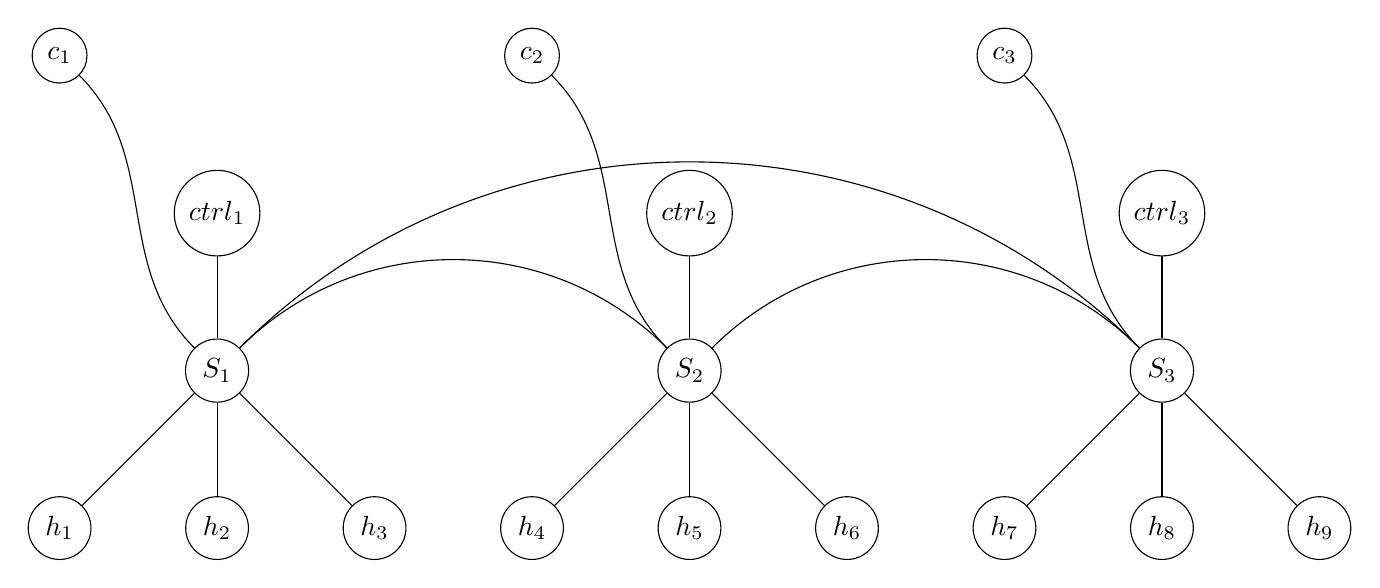
\begin{tikzpicture}[every node/.style={draw, circle}]
    \foreach \n in {1,2,3} {
      \pgfmathsetmacro\x{(\n-2)*6}
      \node (c\n)    at (\x - 2,  4) {$c_\n$};
      \node (ctrl\n) at (\x ,  2) {${ctrl}_\n$};
      \node (S\n)    at (\x ,  0) {$S_\n$};

      \draw (c\n) to[out=315,in=135] (S\n);
      \draw (S\n) -- (ctrl\n);

      \foreach \h in {1,2,3} {
        \pgfmathsetmacro\pos{(\h - 2)*2}
        \pgfmathtruncatemacro\num{((\n - 1)*3) + int(\h)}
        \node (h\num) at (\x + \pos, -2) {$h_{\num}$};
        \draw (S\n) -- (h\num);
      }

    }

    % Links between switches
    \draw (S1) to[out=45,in=135] (S2);
    \draw (S2) to[out=45,in=135] (S3);
    \draw (S1) to[out=45,in=135] (S3);

  \end{tikzpicture}
  \caption{Three switches acting as Paxos nodes.}
  \label{figure:graph.three.switches}
\end{figure}

The point is that these services will be mirrored by the use of our
Paxos--enabled switches.  For our purposes, we will assume that the services
on these hosts are \textit{deterministic}\footnote{Or, more correctly,
\textit{referentially transparent}.} in the sense that the parameters
uniquely determine the state of the service after being processed---if two
hosts running the same service receive the exact same packet, their state
will be identical after having processed it.  This is a prerequisite for our
system.  The OpenFlow switches, running Paxos, will only make sure that
packets are delivered in the \textit{same order} to the end--hosts.

